%!TEX root = ../report.tex
\chapter{Methodology}


\subsection{Formalization of Dynamic Motion Primitives}

\par Dynamic motion primitives use nonlinear differential equations to model the motion primitives. These differential equation is essential represent a damped mass spring system. Attractor landscape of differential equation represent desired kinematic state of the robot. Over the time, various versions of DMPs were presented which were slightly different than one another modified for specific use case or scenario. Following formalization of DMP is taken from \cite{ijspeert2013dynamical}.
A DMP can be represented by following set of equations,  
\begin{equation}\label{DMP_1}
\tau\dot{z} = \alpha_{z}(\beta_{z}(g - y) - z) + f(x)
\end{equation}
\begin{equation}\label{DMP_2}
\tau \dot{y} = z
\end{equation}
and the non-linear function $f(x)$
\begin{equation}\label{forcing_term}
f(x) = \frac{\sum_{i=1}^{N}\psi_{i}(x)w_{i}}{\sum_{i=1}^{N}\psi_{i}(x)}x(g - y_{0})
\end{equation}
where,
\begin{equation}\label{psi}
\psi_{i} = \exp(-{\frac{1}{2\sigma_{i}^{2}}(x - c_{i})^{2}})
\end{equation}
and,
\begin{equation}\label{canonical}
\tau \dot{x} = -\alpha_{x}x
\end{equation}
Equation \ref{DMP_1} and \ref{DMP_2} are the first order representation of a autonomous non-linear second-order differential equation where $f(x)$ is the non-linear term. 
Upon solving these equations, we get state $[\ddot{y}, \dot{y}, y]$ at each time instance. This state represents the acceleration, velocity and position i.e. kinematic state of robotic system. 

If the forcing term is made 0 i.e. $f = 0$, these equations represent a globally stable second-order linear system with $(z, y) = (0, g)$ as a unique point attractor. With appropriate value for $\alpha$ and $\beta$ (with $\beta_{z} = \alpha{z}/4$), the system can be made critically damped in order for $y$ to monotonically converge toward $g$. Such a system implements a stable but trivial pattern generator with $g$ as single point attractor \cite{ijspeert2013dynamical}.

By introducing term $f$, the path followed by system in attractor landscape of differential equation from initial state to the goal state can be modified. This in turn modifies the trajectory followed by mobile robot or robotic manipulator in task-space or joint-space. This non-linear forcing function enables DMP framework to learn almost any arbitrary motion in end-effector space or joint space. It is essentially a weighted sum of equally spaced Gaussian functions denoted by $\psi$ (eq. \ref{psi}) activated at each time step by phase variable $x$. Forcing term $f(x)$ is learned from the demonstrated trajectories. It should be noted that the forcing term $f$ is modified by separation between goal and initial position ($g - y_{0}$), which ensures that the shape of trajectory is also modified by goal separation.

Equation \ref{canonical} is called \textit{canonical system}. $x$ acts as the phase variable modifying forcing term $f(x)$ and hence the shape of the trajectory. It removes the the explicit time dependency of of the system. $x$ initialized at 1 decays to 0 at the end of the motion ensuring convergence to goal state $g$. 

Term $\tau$ is time scaling factor which can be used to modify the speed of execution of the system by modifying the acceleration and velocity term.  

Similar to the above discussed point attractor behavior, DMPs can also learn rhythmic motions exploiting the limit cyclic behavior of non-linear second order differential equation. To achieve rhythmic motion, we need to learn forcing term $f(x)$ which is periodic itself and makes system of equation \ref{DMP_1} and \ref{DMP_2} exhibit limit cyclic behavior. This can be achieved by choosing canonical system to be,

\begin{equation}
	\tau \dot{\phi} = 1
\end{equation}  

where $\phi \in [0, 2\pi]$ is the phase angle of the oscillator in polar coordinates and the amplitude of the oscillation is assumed to be r. Similar to the discrete system, this rhythmic canonical system serves to provide both an amplitude signal $r$ and a phase signal $\phi$ to the forcing term $f$ in equation \ref{DMP_1}.

\begin{equation}
	f(r, \phi) = \frac{\sum_{i=1}^{N}\psi_{i}(x)w_{i}}{\sum_{i=1}^{N}\psi_{i}(x)}r
\end{equation}

\par Point attractor and limit cycle behaviors exhibited by non-linear second order differential equation can be used to model discrete (point to point) and rhythmic motions of robotic arm or mobile platform.   
\vspace{0.5cm}

During this Research and Development project, point attractor DMPs for discrete motion (point-to-point motion) were implemented. For the ease of implementation, above system was slightly modified as follows, 
\begin{equation}\label{actual_DMP}
	\ddot{y} = \tau^{2}\alpha_{y}(\beta_{y}(g-y)-\dot{y}) + f
\end{equation}
\begin{equation}
	\dot{x} = \tau(-\alpha_{x}x)
\end{equation}

This modification does'nt change the properties of original DMP formulation.
\begin{figure}[H]
	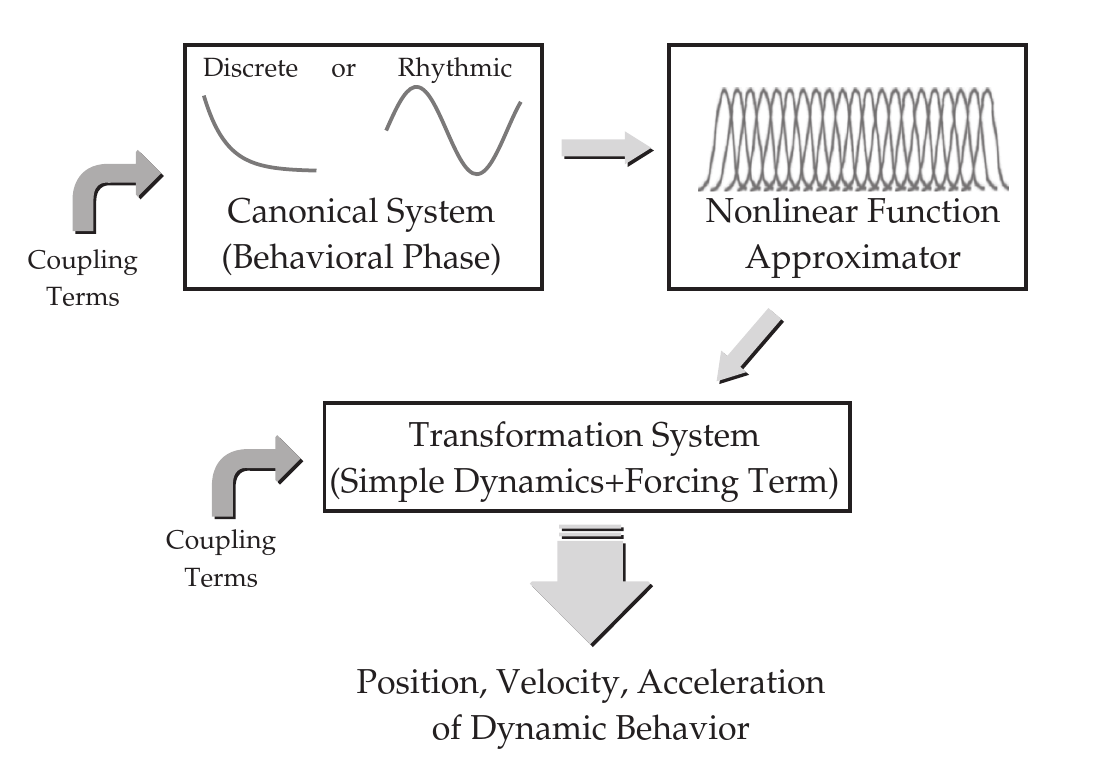
\includegraphics[width=\textwidth]{images/dmp.png}
	\caption{Dynamic Movement Primitive framework}
	\label{fig:DMP_framework}
\end{figure}

\begin{figure}[H]
	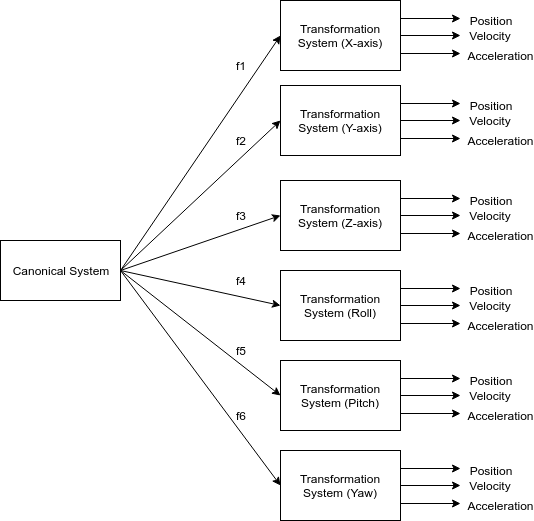
\includegraphics[width=\textwidth]{images/DMP_6DOF.png}
	\caption{Dynamic Movement Primitive framework}
	\label{fig:DMP_6DOF}
\end{figure}


\par Figure \ref{fig:DMP_framework} taken from \cite{ijspeert2013dynamical} show complete DMP framework. 

\subsection{Learning the Motion Primitive from Demonstrated Trajectories}
\par Learning motion primitive means to learn the weights $w_{i}$ in the eq. \ref{forcing_term}. Above system presented in \cite{ijspeert2013dynamical} is linear in the weights $w_{i}$. So variety of learning algorithms can be used. \cite{ijspeert2013dynamical} uses locally weighted regression to learn the weights. 

Desired behavior that should be exhibited by the system is presented as a tuple ($y_{demo}(t)$, $\dot{y}_{demo}(t)$, $\ddot{y}_{demo}(t)$) representing position, velocity and acceleration respectively where $t = [1,2,3,4,....,p]$. Parameter $g$ is goal hence, $g = y_{demo}(t = p)$ and $y_{0} = y_{demo}(t = 0)$. Parameter $\tau$ is temporal scaling factor which needs to adjusted for achieving desired time scaling in the motion. In order to use LWR for estimating $w_{i}$, eq. (\ref{actual_DMP}) can be rearranged to generate function approximation problem as,
\begin{equation}
f = \ddot{y} - \alpha_{z}(\beta_{z}(g - y) - \dot{y})
\end{equation}
Inserting the information from the demonstrated trajectory in the left-hand side of this equation, we obtain,
\begin{equation}
f_{target} = \ddot{y}_{demo} - \alpha_{z}(\beta_{z}(g - y_{demo}) - \tau\dot{y}_{demo})
\end{equation}

While learning the motion primitives, time scaling factor $\tau$ was set to 1 in all the experiments. 

As we have the values $f_{target}$, we can perform a supervised learning to find a best fit for the function represented by $f_{target}$. 

Locally weighted regression finds for each kernel function $\psi_{i}$ in $f$, the
corresponding $w_{i}$, which minimizes the locally weighted quadratic error criterion,

\begin{equation}
	J_{i} = \sum_{t=1}^{p}\psi_{i}(t)(f_{target}(t)-w_{i}\xi(t))^{2}
\end{equation}

where $\xi_{i} = x(t)(g-y_{0})$ for the discrete system and $\xi_{i} = r$ for rhythmic system. Solution to above linear regression problem is,

\begin{equation}
	w_{i} = \frac{s^{T}\Gamma_{i}f_{target}}{s^{T}\Gamma_{i}s}
\end{equation}

where,\\
\\
\vspace{1cm}
$
s = 
\begin{pmatrix}
\xi(1) \\
\xi(2) \\
\vdots  \\
\xi(p) 
\end{pmatrix}
$
$
\Gamma = 
\begin{pmatrix}
	\psi_{i}(1) &   &  & 0 \\
	 &\psi_{i}(2)&  &  \\
	 &  & \ddots &   \\
	0 &  &  & \psi_{i}(p)
\end{pmatrix}
$
$
f_{target} = 
\begin{pmatrix}
f_{target}(1) \\
f_{target}(2) \\
\vdots  \\
f_{target}(p) 
\end{pmatrix}
$


 

After 

 




\subsection{Inverse Kinematics Solver and Trajectory Controller}

In order to execute the task-space trajectory generated by DMP framework, Cartesian velocities are needed to be converted to the joint velocities with the help of inverse kinematic solver. Robot arm used in the experiments (KUKA YouBot arm) has five degrees of freedom. Five degrees of freedom are not sufficient to carry out 6 degrees of freedom cartesian motion. Due to this design deficiency, manipulator is always in the singular configuration. It is well-known that when a manipulator is at-or is in the neighborhood of a singular configuration, severe restrictions may occur on its motion. To overcome this situation, \textit{weighted damped least square pseudo inverse method} for computing joint velocities was chosen. This method allows us to loose the constraints on individual degrees of freedom in task-space. Which allowed us to ignore velocity constraints on 3 rotational degrees of freedom. This is called user-defined accuracy method to control the manipulator. \cite{chiaverini1994review}
\\
The relation between joint space and task space velocity can be given by, 

\begin{equation}\label{theta_dot}
	v = J(\theta) \dot{\theta} 
\end{equation}

\begin{equation}
	\dot{\theta} = J(\theta)^{-1}  v
\end{equation} 
Where, \\
$J(\theta)$ is jacobian of manipulator, \\
$v$ is task space velocity vector, \\
$\dot{\theta}$ is joint space velocity vector. \\

When manipulator is near a singularity, sigma  large joint velocities may occur or degenerate directions may exist where end-effector velocity
is not feasible\cite{chiaverini1994review}. To overcome this situation, damped least square method can be used where a degraded solution is generated near the singularities proposed in \cite{wampler1986manipulator, nakamura1986inverse}.  

\begin{equation}
	J^{T}(\theta)v = (J^{T}(\theta)J(\theta) + \lambda ^{2}I)\dot{\theta}
\end{equation}

Where, \\
$\lambda > 0 $ is the damping factor, and \\
$I $ is identity matrix. \\

Solution to above problem can be given by, 
\begin{equation}\label{damped_least_sol}
	\dot{\theta} = (J^{T}(\theta)J(\theta) + \lambda^{2}I)^{-1}J^{T}(\theta)v
\end{equation} 

It should be noted that, if the value of $\lambda$ in eq. \ref{damped_least_sol} is set to 0, eq. \ref{damped_least_sol} reduces to eq. \ref{theta_dot}.

The effect of value of lambda on joint velocities can be analyzed in detail by singular value decomposition of the Jacobian matrix and that is, 

\begin{equation}
	J = \sum_{i=1}^{6}\sigma_{i}u_{i}\textbf{v}_{i}^{T}
\end{equation} 

Using singular value decomposition, equation \ref{damped_least_sol} can be re-written as,

\begin{equation}
\dot{\theta} = \sum_{i=1}^{6}\frac{\sigma_{i}}{\sigma_{i}^{2} + \lambda^{2} }\sigma_{i}u_{i}\textbf{v}_{i}^{T}v
\end{equation} 

It can be observed in above equation that if $\sigma \gg \lambda$, then $\lambda$ has practically no effect on joint velocities. But if $\sigma$ is close to zero, then the joint velocities are greatly affected by value of $\lambda$.  

Since the arm has only five degrees of freedom, it is always in singular configuration and hence it is not possible to execute the 6 degrees of motion at all the time instances. This situation can be overcome by ignoring motion in 3 rotational degrees of freedom with the help of the method called \textit{weighted damped least square pseudo inverse}. In this method, 	
\section{Setup}


\section{Experimental Design}
